\section{Software}
Softwaren til \textit{The Cell Collector} udvikles i Matlab. Programmet udvikles af modulær kode, der afgrænser de enkelte funktionaliteter. Ved objektorienteret programmering beskrives koden typisk vha. klassediagrammer og 3-lags modellen, hvor de enkelte klassers ansvar og grænseflader tydeligt er defineret. Da Matlab kode er opdelt i funktioner fremfor for klasser er modellen ikke velegnet. I stedet beskrives softwaren vha. blokdiagrammer, hvor funktionernes opbygning og relationer med hinanden er vist. 

Blokdiagrammet (figur: \ref{fig:bdd_software}) viser hvordan programmet er opdelt i blokke, som afgrænser de enkelte funktionaliteter. Blokkene i det nederste lag skal ses som ækvivalente til funktioner i Matlab.  
De overordnede blokke i programmet er:
\begin{itemize}
\item Arduino
\item Kamera
\item User Interface
\end{itemize}

Disse blokke er nærmere beskrevet under hver deres afsnit.

\begin{figure}[H]
	\centering
	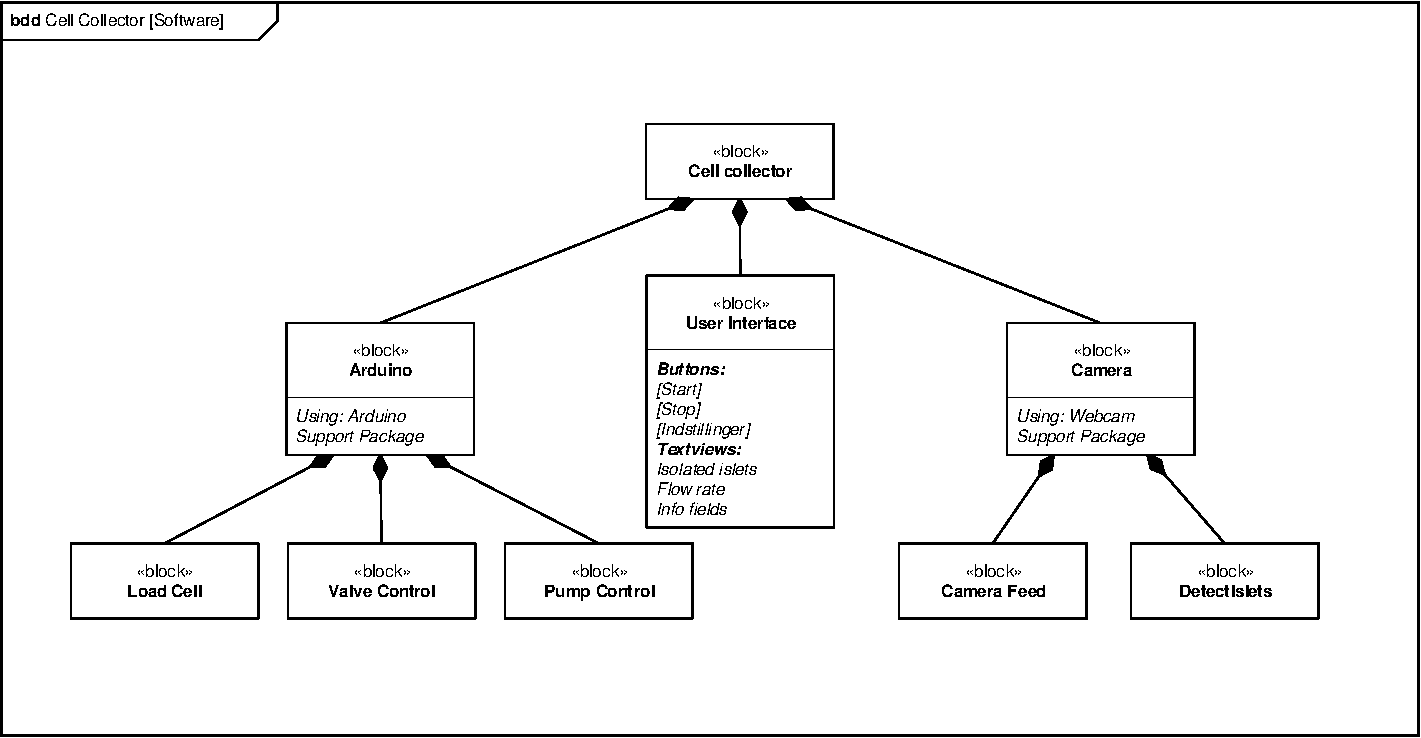
\includegraphics[width=1\textwidth]{billeder/BDD_Software-crop.pdf}
	\caption{BDD - Cell Collector [Software]}
	\label{fig:bdd_software}
\end{figure}


\subsection{Arduino}
Denne bloks formål er, at håndtere al funktionalitet til styring af Arduinoen. Til styring af Arduinoen anvendes Arduino Support Package, som frit kan hentes hos Mathworks. Den indeholder basale funktioner til bl.a. opsamling af analoge signaler, understøttelse af digitalt og PWM output og styring af DC motorer. Support biblotektet indeholder de funktioner der skal til for at styre systemets hardware.
For at initialisere Arduinoen og hardwaren implementeres en funktion, som opsætter Arduinoen med de inputs og outputs der er specificeret under hardware afsnittet (figur: \ref{ibd_Hardware}, s. \pageref{fig:ibd_Hardware}). Denne funktion er kaldt initArduino. Når brugeren klikker "Stop" skal systemet lukke ned som specificeret i Use Case 3: Stop sorteringscyklus (s. \pageref{uc:3}). Til dette implementeres en funktion kaldet stopArduino. 

\newpage

Arduino blokken er yderligere opdelt i 3 underkategorier, som vist i figur \ref{fig:bdd_software}. I det interne blok diagram (figur: \ref{fig:ibd_software_arduino}) ses underblokkenes relationer med hinanden. Disse blokke er nærmere beskrevet herunder.  
\begin{figure}[H]
	\centering
	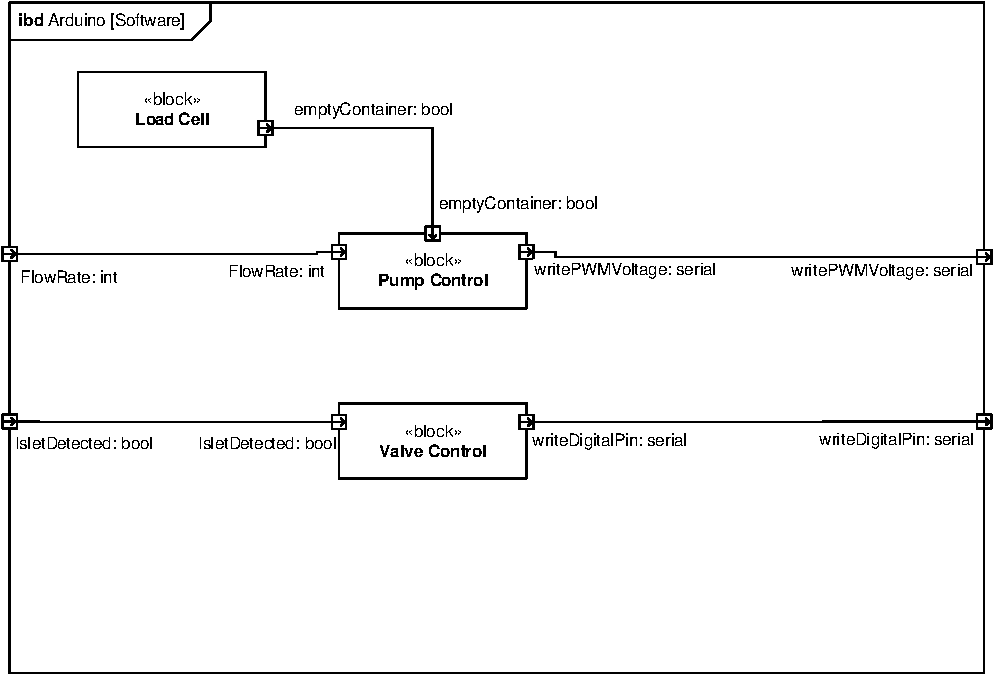
\includegraphics[width=1\textwidth]{billeder/IBD_Software_Arduino-crop.pdf}
	\caption{IBD - Arduino [Software]}
	\label{fig:ibd_software_arduino}
\end{figure}
\subsubsection{LoadCell}
Denne funktion anvendes til, at få feedback fra loadcellen. Den læser det analoge input fra Arduinoen og sammenligner den med grænseværdien for hvornår celleopløsningsbeholderen er tom. Funktionens output er en boolean, som enten er true eller false alt efter om celleopløsningsbeholderen er tom.
\subsubsection{Pump Control}
I denne funktion implementeres alt funktionalitet til styring af pumpen. Funktionen har en integer værdi som input, der specificerer flow hastigheden. Output af funktionen er et PWM moduleret signal til, at justere hastigheden på pumpen. Til dette anvendes funktionen writePWMVoltage fra Arduino Support pakken.
\subsubsection{Valve Control}
Funktionen til styring af ventilen har en boolean som input. Denne værdi indikerer om en Langerhansk Ø er detekteret af kameraet. Alt efter værdien af denne sættes forbindelsen til ventilen høj eller lav med funktionen writeDigitalPin. 

\newpage
\subsection{Kamera}
Denne bloks formål er, at modtage et feed fra kameraet samt at detektere om en Langerhansk Ø har passeret kameraet. Som det ses på det overordnede blok diagram for softwaren (figur: \ref{fig:bdd_software}) består kamera blokken af 2 underblokke. Nedenstående interne blok diagram (figur: \ref{fig:ibd_software_camera}) viser, hvordan disse blokke er forbundet internt. De enkelte blokkes funktion er yderligere beskrevet herunder.
\begin{figure}[H]
	\centering
	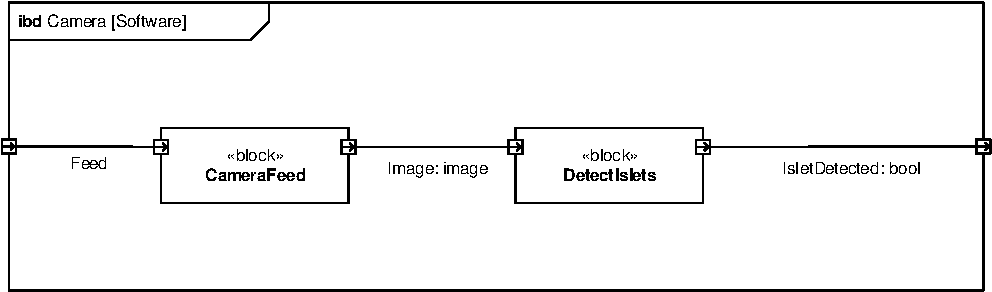
\includegraphics[width=1\textwidth]{billeder/IBD_Software_Kamera-crop.pdf}
	\caption{IBD - Camera [Software]}
	\label{fig:ibd_software_camera}
\end{figure}

\subsubsection{CameraFeed} \label{subsub:Dcamerafeed}
Denne bloks funktion er at modtage feedet fra kameraet og gemme billedet i handles. Til dette anvendes funktionen snapshot, der gemmer det nuværende billede som en variabel.  
\subsubsection{DetectIslets}
I denne funktion foregår alt billedbehandlingen på det omsamlede billede. Billedet segmenteres for at fjerne støj og andet væv. Alt efter om en Langerhansk Ø er detekteret eller ej returneres true eller false. 

\newpage
\subsection{Funktioner}
I nedenstående liste er systemets funktioner opsummeret. 
\begin{itemize}
\item initArduino
\item pumpControl 
\item valveControl 
\item loadCell 
\item cameraFeed 
\item detectIslets 
\end{itemize}
Herudover skal systemets indstillinger kunne ændres, samt data om sorteringscyklussen skal logges. Til dette implementeres funktionerne settings og exportData 
\begin{itemize}
\item settings 
\item exportData 
\end{itemize}

\newpage
\subsection{User Interface}
\subsubsection{Hovedvindue}
I figur \ref{fig:gui} er et Mockup af GUI'en vist. I venstre side er der placeret en \textit{Start knap}, som skifter stadie til en \textit{Stop knap} når den er klikket. Under denne knap er en række indikatorer placeret til, at give operatøren feedback om status omkring initialiseringen af Hardwaren. 
I højre side af GUI'en er der placeret tekstfelter til, at give brugeren feedback omkring den nuværende sorteringscyklus, samt de anvendte indstillinger. Under disse felter er en knap til \textit{Indstillinger}. Når denne klikkes åbnes et nyt vindue, hvor operatøren kan ændre i indstillingerne. 
\begin{figure}[H]
	\centering
	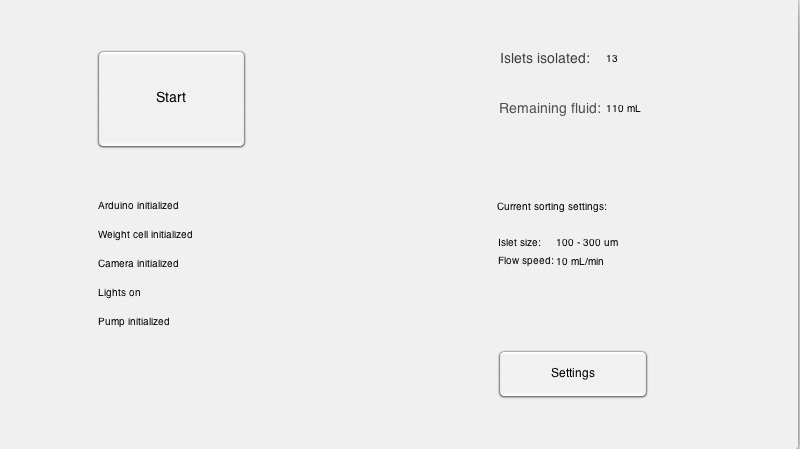
\includegraphics[width=1\textwidth]{billeder/GUI.png}
	\caption{Mockup af GUI}
	\label{fig:gui}
\end{figure}

\newpage
\subsubsection{Indstillinger}
I figur \ref{fig:gui_settings} er et Mockup af \textit{Indstillingsvinduet} vist. Via 2 tekstfelter har operatøren mulighed for, at ændre størrelsen for de celler som systemet skal sorterer. Herudover har operatøren via en dropdown menu mulighed for at ændre flowhastigheden for pumpen. I Indstillingsvinduet er der yderligere placeret en "Annuller" knap og en "Gem Indstillinger" knap.
\begin{figure}[H]
	\centering
	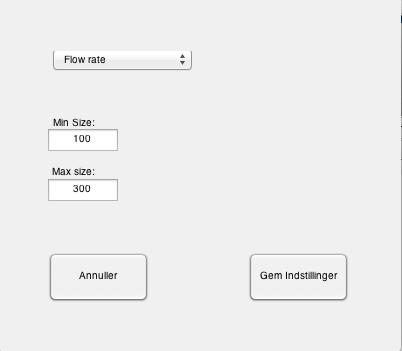
\includegraphics[width=0.5\textwidth]{billeder/GUI_settings.png}
	\caption{Mockup af Indstillinger}
	\label{fig:gui_settings}
\end{figure}


\newpage
\subsubsection{Callbacks}
For de 3 knapper i GUI'en oprettes der 3 callback funktioner, hvor forskellig kode eksekveres når knapperne klikkes. Disse 3 callback funktioner er nærmere beskrevet herunder bl.a. vha. flow chart diagrammer.
\subsubsection{Start Callback}
Denne callback funktion kaldes når operatøren klikker på Start knappen på GUI'en. Flowet i callbacket er vist i figur \ref{fig:act_start}.
\begin{figure}[H]
	\centering
	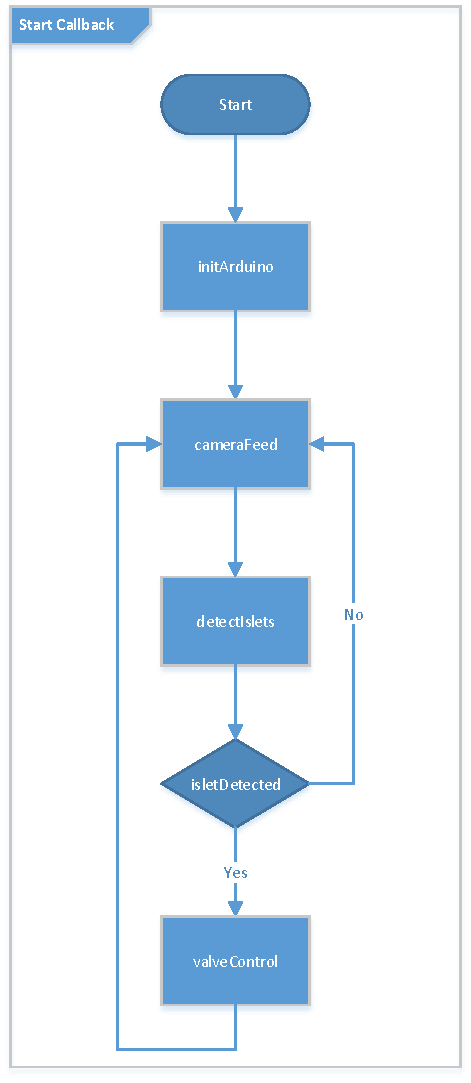
\includegraphics[width=0.5\textwidth]{billeder/act_start-crop.pdf}
	\caption{Flowchart diagram for Start Callback}
	\label{fig:act_start}
\end{figure}

\newpage
\subsubsection{Stop Callback}
Denne callback funktion kaldes når operatøren klikker på Stop knappen på GUI'en. Flowet i callbacket er vist i figur \ref{fig:act_stop}.
\begin{figure}[H]
	\centering
	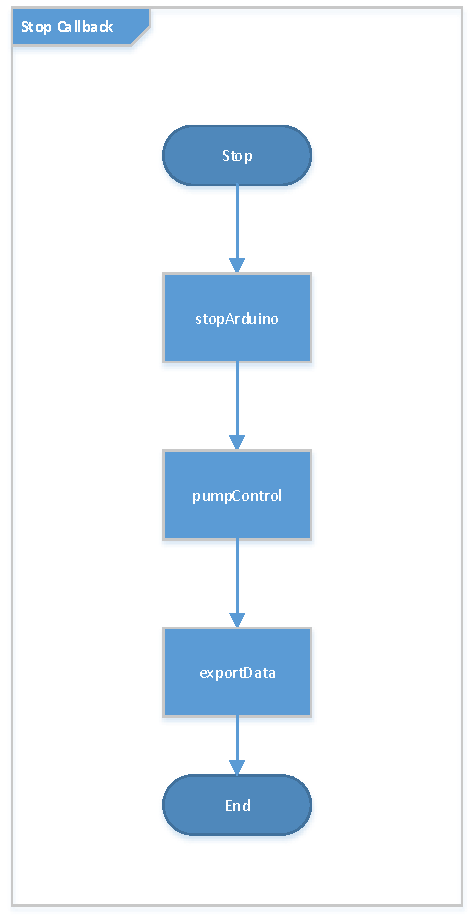
\includegraphics[width=0.5\textwidth]{billeder/act_stop-crop.pdf}
	\caption{Flowchart diagram for Stop Callback}
	\label{fig:act_stop}
\end{figure}

\newpage
\subsubsection{Indstillinger Callback}
Denne callback funktion kaldes når operatøren klikker på Settings knappen på GUI'en. Flowet i callbacket er vist i figur \ref{fig:act_settings}. Når knappen klikkes åbnes et nyt vindue, hvor systemets indstillinger kan ændres. De ændrede indstillinger anvendes i funktionerne detectIslets og pumpControl. 
\begin{figure}[H]
	\centering
	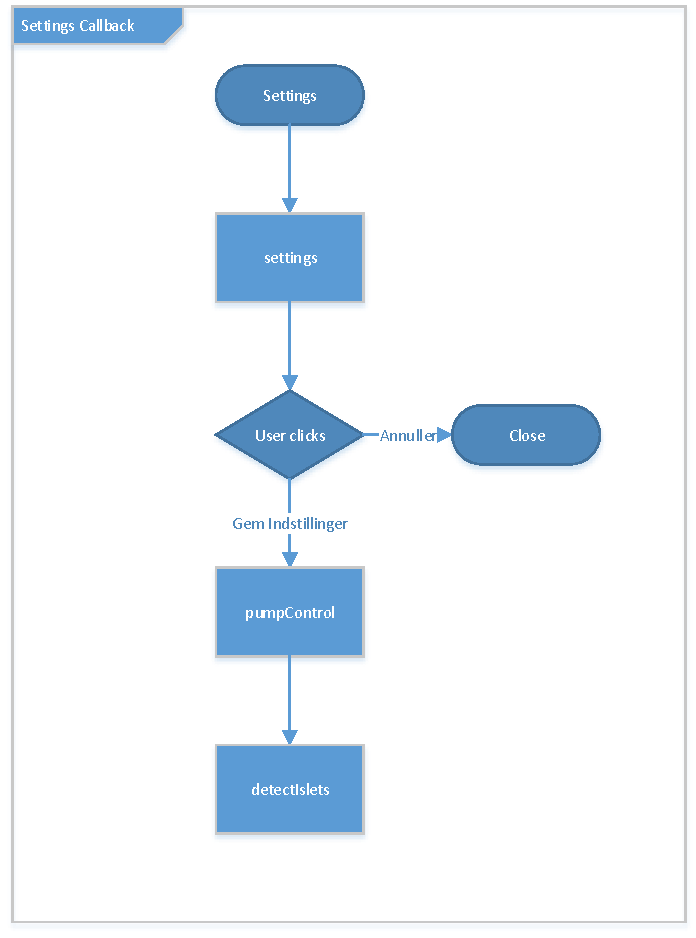
\includegraphics[width=0.5\textwidth]{billeder/act_settings-crop.pdf}
	\caption{Flowchart diagram for Settings Callback}
	\label{fig:act_settings}
\end{figure}







